\documentclass[conference]{IEEEtran}
\usepackage[english]{babel}
\usepackage{geometry}
\usepackage{amsmath}
\usepackage{amsthm}
\usepackage{graphicx}
\usepackage{caption}
\usepackage[utf8]{inputenc}


%%%%%%%% SUB-FIGURE PACKAGE
\usepackage{subcaption}

%%%%%%%% MULTI-COLUMNS PACKAGE
\usepackage{multicol}

%%%%%%%% PERSONAL COMMANDS
\usepackage{amssymb}

%%%% Important sets
\renewcommand{\O}{\mathbb{O}}
\newcommand{\N}{\mathbb{N}}
\newcommand{\Z}{{\mathbb{Z}}}
\newcommand{\Q}{{\mathbb{Q}}}
\newcommand{\R}{{\mathbb{R}}}

%%%% Usual operations
\newcommand{\pow}[2]{#1^{#2}}
\newcommand{\expp}[1]{e^{#1}}
\newcommand{\fst}{\mathrm{fst}}
\newcommand{\snd}{\mathrm{snd}}

%%%% Lambda Calculus
\newcommand{\dneq}{\,\, \# \,\,}
\newcommand{\prm}[1]{\mathrm{\mathbf{#1}}}
\renewcommand{\S}{\prm{S}}
\newcommand{\I}{\prm{I}}
\newcommand{\K}{\prm{K}}
\newcommand{\ch}[1]{\ulcorner #1 \urcorner}

%%%% Ordinal Lambda Calculus
\newcommand{\ordAlph}{\Sigma_{\text{Ord}}}
\newcommand{\termOrd}{\text{Term}_\text{Ord}}
\newcommand{\fl}{\mathrm{fl}}
\newcommand{\sk}{\mathrm{sk}}

%% Superscript to the left
% https://latex.org/forum/viewtopic.php?t=455
\usepackage{tensor}
\newcommand{\app}[3]{\tensor*[^{#1}]{\left(#2, #3\right)}{}}

%%%% Make optional parameter
% https://bit.ly/3jVGRwQ
\usepackage{xparse}

%%%% Statistics
\NewDocumentCommand{\E}{o m}{
  \IfNoValueTF{#1}
  {\mathbb{E}\left[#2\right]}
  {\mathbb{E}^{#1}\left[ #2\right]}
}
\NewDocumentCommand{\V}{o m}{
  \IfNoValueTF{#1}
  {\mathrm{Var}\left[#2\right]}
  {\mathrm{Var}^{#1}\left[ #2\right]}
}
\RenewDocumentCommand{\P}{o o m}{
  \IfNoValueTF{#1}
  {\IfNoValueTF{#2}
    {\mathrm{P}\left(#3\right)}
    {\mathrm{P}^{#2}\left(#3\right)}}
  {\IfNoValueTF{#2}
    {\mathrm{P}_{#1}\left(#3\right)}
    {\mathrm{P}_{#1}^{#2} \left(#3\right)}}
}

%%%% Lambda Calculus
\NewDocumentCommand{\cx}{o}{
  \IfNoValueTF{#1}
  {\left[\quad\right]}
  {\left[\, #1 \,\right]}
}

%%%% Create absolute value function
% https://bit.ly/33Rkq6H
\usepackage{mathtools}
\DeclarePairedDelimiter\abs{\lvert}{\rvert}%
\DeclarePairedDelimiter\norm{\lVert}{\rVert}%
\makeatletter
\let\oldabs\abs
\def\abs{\@ifstar{\oldabs}{\oldabs*}}
%
\let\oldnorm\norm
\def\norm{\@ifstar{\oldnorm}{\oldnorm*}}
\makeatother

%%%%%%%% LOGIC TREES
\usepackage{prftree}

%%%%%%%% SPLIT EQUATIONS
% https://bit.ly/33P1OUM
\allowdisplaybreaks

%%%%%%%% FLOAT SPECIFIER
% https://bit.ly/30Wi4BC
\usepackage{float}

%%%%%%%% TO USE SHORT COMMANDS FOR VECTOR LINES
\usepackage{esvect}

%%%%%%%% DIFFERENT FONTS FOR MATH
\usepackage{mathrsfs}

%%%%%%%% FOOTNOTE STUFF
\renewcommand{\thefootnote}{\fnsymbol{footnote}}



%%%%%%%% MARGIN
\geometry{verbose, letterpaper, tmargin=3cm,
  bmargin=3cm,lmargin=2.5cm,rmargin=2.5cm}

%%%%%%%% PARAGRAPH SETTINGS
% https://bit.ly/36WrtN4
\setlength\parindent{0pt}

% https://bit.ly/371dvto
\setlength{\parskip}{5pt}

%%%%%%%% HYPERREF PACKAGE
\usepackage{hyperref}
\hypersetup{linkcolor=blue}
\hypersetup{citecolor=blue}
\hypersetup{urlcolor=blue}
\hypersetup{colorlinks=true}


%%%%%%%% BIB-LATEX STUFF
\usepackage[style=ieee,
            bibstyle=ieee,
            citestyle=ieee,
            hyperref=true,
            backend=biber]{biblatex}
\addbibresource{ref.bib} %Put relative path to ref

%%%%%%%% DEFINITION AND THEOREM DEFINITIONS
\theoremstyle{definition}
\newtheorem{definition}{Definition}[section]

\theoremstyle{remark}
\newtheorem{remark}{Remark}

\theoremstyle{remark}
\newtheorem{question}{Question}

\newtheorem{theorem}{Theorem}[section]


%%%%%%%% CODE RENDERING !!! UNCOMMENT IF NEEDED !!!
% Compile with flag -shell-escape
%\usepackage{minted}

%%%%%%%% START DOCUMENT
\title{Supervised Learning for Psychological Attention to High School Students}

\author{\IEEEauthorblockN{Juan S. Cárdenas-Rodríguez}
  \IEEEauthorblockA{\textit{Department of Mathematical Sciences} \\
    \textit{EAFIT University}\\
    Medellín, Colombia \\
    jscardenar@eafit.edu.co} \and \IEEEauthorblockN{David Plazas}
  \IEEEauthorblockA{\textit{Department of Mathematical Sciences} \\
    \textit{EAFIT University}\\
    Medellín, Colombia \\
    dplazas@eafit.edu.co} }


\begin{document}
\maketitle

%%%%%%%%%%%%%%%%%%%%%%%%%%%%%
\begin{abstract}
  Hello.
\end{abstract}

\begin{IEEEkeywords}
  Nice.
\end{IEEEkeywords}
%%%%%%%%%%%%%%%%%%%%%%%%%%%%%

\textit{Note}: All the code and the latex file can be found in
\href{https://github.com/juanscr/ai-works}{the GitHub repository}.

\section{Introduction}

Mental health is crucially important for every human being and has become one of
the most important issues surrounding human health. According to the World
Health Organization (WHO)\footnote{WHO's \href{https://bit.ly/34l2v94}{2001
    report.}} report of 2001, mental disorders can affect 25\% of the
population, therefore, suggesting the ongoing trend of people suffering from
lack of mental health. Additionally, with the recent events caused by the
COVID-19 pandemic, mental issues have risen as consequence of lockdowns all
around the globe, as have been proved by recent studies
\parencite{rossi2020,xiong2020}.

Furthermore, mental health is more important to monitor in adolescents and kids
as this group is in the process of developing their mental structure and
character. In this manner, as they continue creating their view about the world
they must be surrounded by a healthy environment that promotes healthy habits
and relationships with their surroundings.

As a result, schools and parents have an important responsibility to the
students of creating this environment and wisely handling mental health issues.
However, high schools do not always know how to handle or detect cases of mental
health issues. Additionally, technology has led to targeted harassing becoming
more popular over time, therefore, complicating the probability of detecting
these cases.

Some of the most common and important mental health issues are anxiety,
depression, and hyperkinetic disorder. According to \textcite{schulte2016},
around 10\% to 20\% of children suffer from hyperkinetic disorder. Additionally,
school teachers just assume this disorder is a cause of undisciplined students
and can take the hyperkinetic student to a depressive state. These three mental
disorders can leave severe damage to a kid and can lead them to suicide.

Hence, it is of the utmost importance to quickly and efficiently detect students
that might be having a mental health issue to immediately start a process with
him/her. Furthermore, this detection has to be done with measurable variables
that can be easily obtained from questionnaires or school data.

The present work is oriented to the application of supervised learning
techniques (decision trees, support vector machines and neural networks) for
classifying the data from the survey, aiming for the construction of a model to
detect individuals with mental health issues. Recent developments and the
increasing popularity of supervised techniques has contributed to their
application in different areas, among them, mental health.

The novel work by \textcite{thieme2020} makes and excellent literature review of
Machine Learning (ML) in mental health, including the current state-of-the-art
and formulates new strategies for integrating human-oriented research with
multi-disciplinary. They also conclude that ML applied in mental health is
``still in its infancy'' given the complexity and difficulties of constructing
robust models for clinically reliable outputs.

Additionally, the work presented by \textcite{shatte2019} is also a complete
compendium of recent ML applications in mental health, including the usage
of Support Vector Machines (SVMs), Decision Trees (DTs), Neural Networks (NN)
and beyond. This paper includes a systematic review of over three hundred papers
and it concludes that these techniques have brought benefits
across the areas of diagnosis, treatment, research and clinical administration.

Finally, another overview of applications of Artificial Intelligence (AI) for Mental
Illnesses is the research published by \textcite{graham2019}, where the authors
reviewed 28 research papers which include modern methodologies (and
technologies) for predicting or classifying psychological illnesses such as
depression, schizophrenia or suicidal behavior. The study discusses how the
application of AI techniques supports the clinical practice while considering its
limitations, it also presents some ethical implications and states which areas need
further development.

This document is organized as
follows: Section \ref{sec:meth} shows the general methodology used in this work,
moreover Section \ref{sec:res} shows the obtained results over the data and
slight modifications, finally Section \ref{sec:conc} concludes this work and
sets pillars for future works.

\section{Methodology}\label{sec:meth}
All the code developed for this work was implemented in Julia 1.5.3. and
can be found in the authors'
\href{https://github.com/juanscr/ai-works}{GitHub repository}.

\subsection{Survey}
The used survey for extracting data was initially designed for developing
a Fuzzy Inference System, but the data was labeled according to
unsupervised clustering techniques, obtaining 2 clusters through the subtractive
algorithm \parencite{chiu1994} and then sharpened using Fuzzy-C-Means
\parencite{dunn1973}. The data has 6 variables and 113 observations. This
dataset was divided with the standard $60-20-20$ rule, creating a training
dataset with $60\%$ of the complete data, a validation set with $20\%$ and a
test set with $20\%$ as well. All data was normalized by dividing each dimension
by its maximum (in absolute value), casting the data into the [-1,1] hypercube.

\subsection{Support Vector Machines}
\textcite{burges1998} published an excellent reference for the theoretical
background on SVMs with different kernels and explains the formulation of the
optimization problem. The SVMs were used directly from Scikit-Learn
\parencite{scikit-learn, sklearn_api} using
\href{https://bit.ly/3lDHADX}{Julia's API}. The SVMs were trained using three
different kernels: linear, polynomial and RBF (radial base function).

\subsection{Decision Trees}
We refer to \textcite{bramer2007} for the general ideas behind the decision tree
classifier.

\subsection{Neural Networks}
The book of \textcite{aggarwal2018} was used as primary reference for the
formulation of the NN learning machine and the details of its implementation,
such as the backpropagation algorithm and the bias correction.
The NN was implemented by the authors, including the bias correction and the
momentum acceleration term.

The NNs trained used a fully-connected Multi-Layer Perceptron (MLP) using
different number of neurons and different learning rates. The detailed process
will be now described: let $L$ be the number of hidden layers in the MLP and let
$\mathcal{L}\in\mathbb{R}^{L}$ be a vector containing the number of neurons on
each hidden layer. The number of hidden layers was varied as $L=1,2,3$ and let
$l_i$ be the number of neurons in the $i$-th layer of the MLP, hence, each
$l_i\in\mathcal{L}$ was varied in $1,2,3$ as well. This gives a total of
$3^1+3^2+3^3=39$ different permutations just for the architecture of the MLP,
and this was repeated for learning rates as $\eta=0.2,0.5,0.9$, yielding a total
of $117$ NNs to be trained.

All $117$ MLPs were trained sequentially, fixing a maximum of 50 epochs,
and only the main results for the two bests and for the worst MLP configurations
will be presented, in order to keep this paper concrete. The order relation
between the trained NNs was established by evaluating the cost function at the
end of the final epoch. All MLPs used the sigmoid activation function.

The results are presented using three learning curves: the sum of local
gradients per layer at the end of each epoch, the average error energy and a
Receiver Operating Characteristic (ROC) curve, comparing the obtained results
with the real labels.
\begin{itemize}
  \item The sum of gradients per layer at the end of each epoch is an approach
  visualizing if the training algorithm is solving the optimization problem,
  since the sum of local gradients must converge to zero as each gradient
  converges to zero. It is well-known that the vanish of gradients is a
  necessary condition for optimality and the training algorithm is just an
  optimization problem minimizing the output error (cost function).
  \item The average error energy is the cost function of the optimization
  problem. Let $y_i\in\mathbb{R}^n$ be the real output of a given input pattern
  $x_i\in\mathbb{R}^m$ and let $\hat{y}_i\in\mathbb{R}^n$ be the output of the
  NN for the same input pattern. Denoting each component by superscripts, the
  average error energy $\xi_{av}$ on each epoch is then computed as
  \begin{equation}
    \xi_{av}=\dfrac{1}{2}\sum_{i=1}^{N}\sum_{k=1}^n\left(y^k_i-\hat{y}^k_i\right)^2,
  \end{equation}
  where $N$ is the training sample size. Thus, it is clear that
  $\xi_{av}\rightarrow0$ as the training algorithm solves the learning problem
  well.
  \item The ROC curve is a tool that helps visualize the correct classifications
  of the learning machine by plotting the true positive rate on the vertical
  axis, and false positive rate on the horizontal axis. The Area Under the Curve
  (AUC) is an indicator of how good the data is being classified by the model,
  with higher values being better usually better.
\end{itemize}

\section{Results}\label{sec:res}
For giving an idea of the dataset treated in this work (visualization), the data
was embedded into a 2-dimensional space using the T-student Stochastic
Neighborhood Embedding (TSNE) \href{https://github.com/lejon/TSne.jl}{in Julia}
\parencite{maaten2008}. In Fig. \ref{fig:emb_dat}, the embedded dataset is
presented.
\begin{figure}
  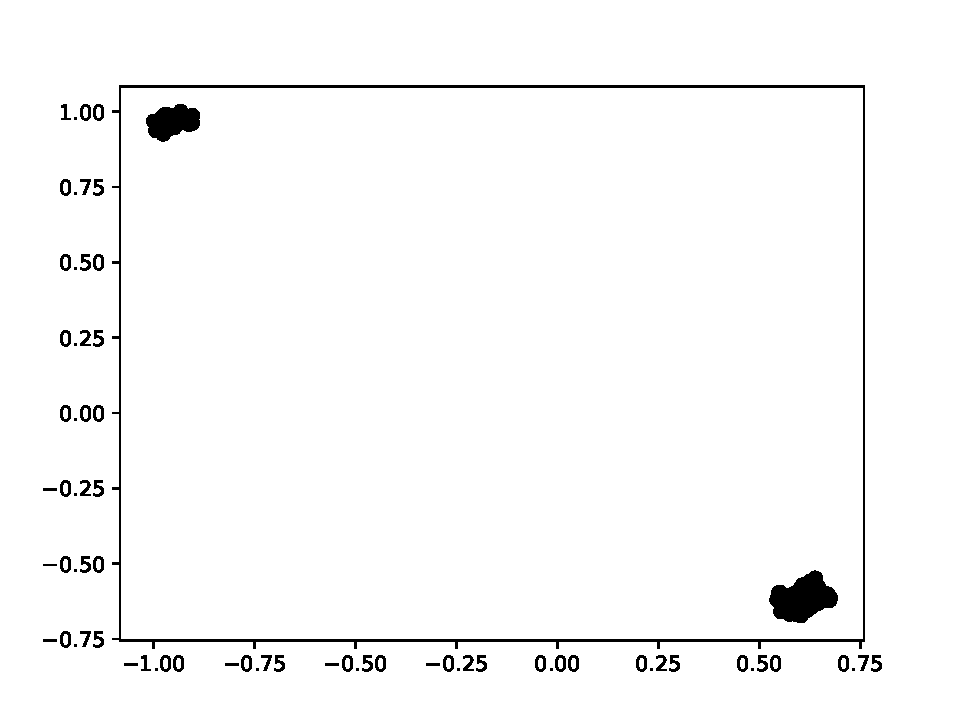
\includegraphics[width=\columnwidth]{figs/embedded-data.pdf}
  \caption{Embedded dataset.}
  \label{fig:emb_dat}
\end{figure}

\subsection{Support Vector Machines}

\subsection{Decision Trees}
\begin{figure}
    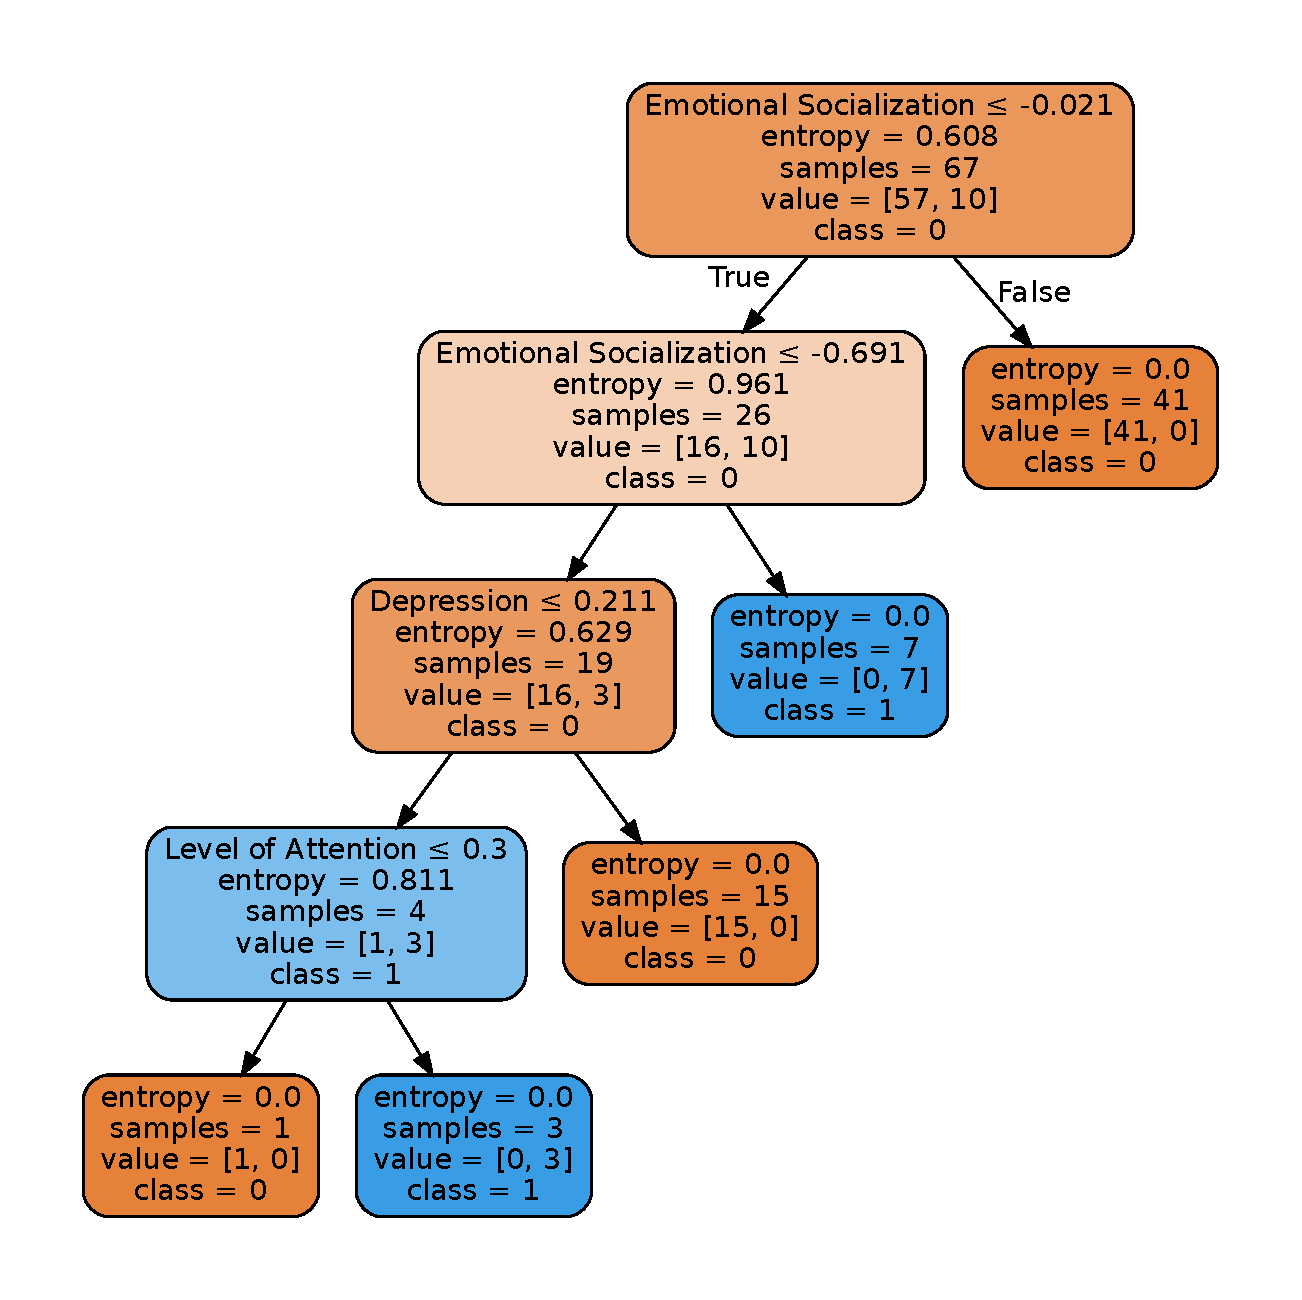
\includegraphics[width=\columnwidth]{figs/tree-graph.pdf}
    \caption{Decision tree.}
    \label{fig:dt}
\end{figure}

\begin{figure*}
    \centering
    \begin{subfigure}[b]{0.32\textwidth}
        \centering
        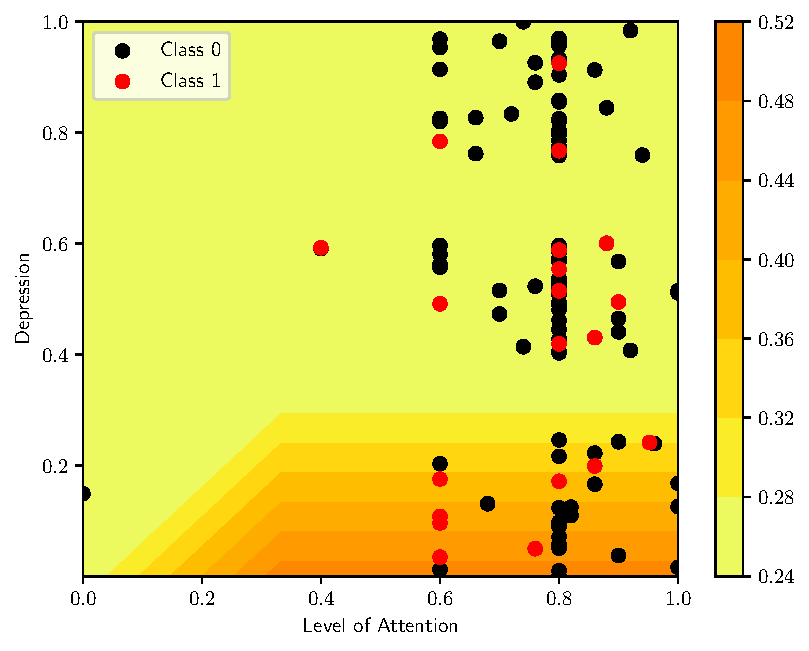
\includegraphics[width=\textwidth]{figs/tree-contour-0-3.pdf}
        \caption{}
    \end{subfigure}
    \begin{subfigure}[b]{0.32\textwidth}
        \centering
        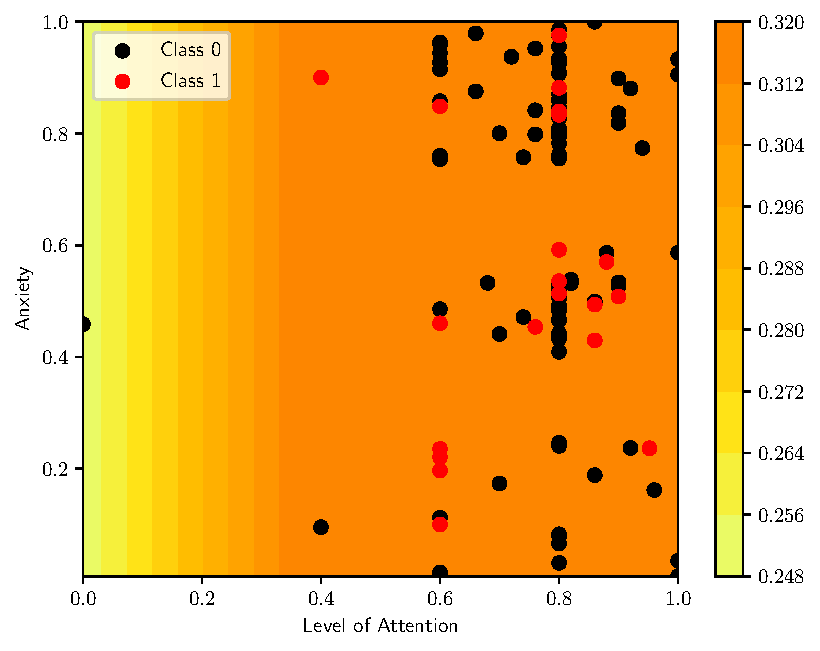
\includegraphics[width=\textwidth]{figs/tree-contour-0-4.pdf}
        \caption{}
    \end{subfigure}
    \begin{subfigure}[b]{0.32\textwidth}
        \centering
        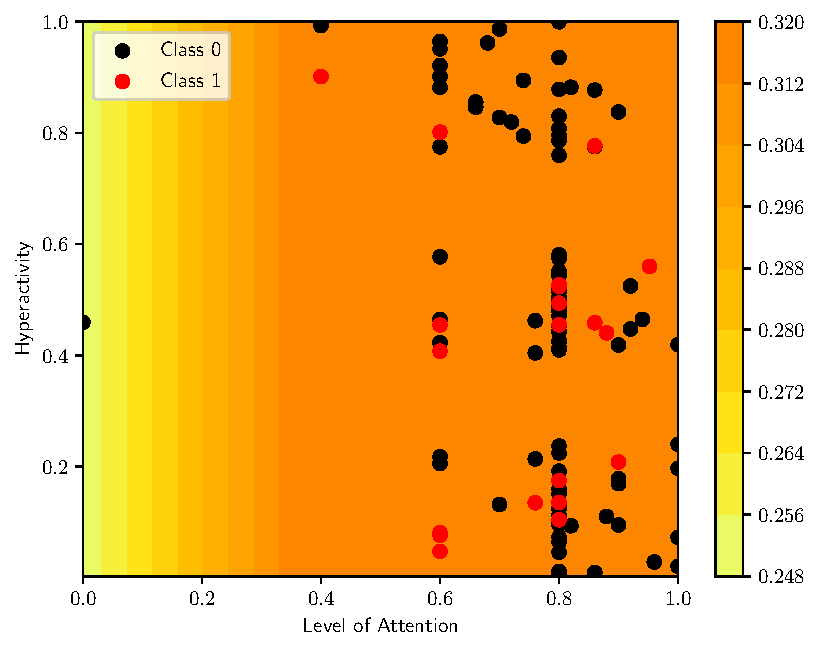
\includegraphics[width=\textwidth]{figs/tree-contour-0-5.pdf}
        \caption{}
    \end{subfigure}

    \begin{subfigure}[b]{0.32\textwidth}
        \centering
        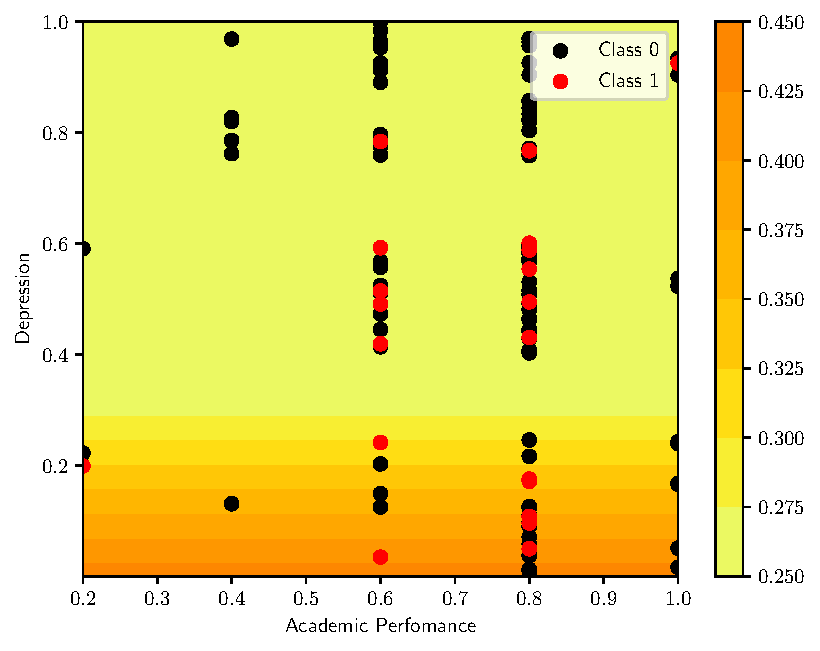
\includegraphics[width=\textwidth]{figs/tree-contour-1-3.pdf}
        \caption{}
    \end{subfigure}
    \begin{subfigure}[b]{0.32\textwidth}
        \centering
        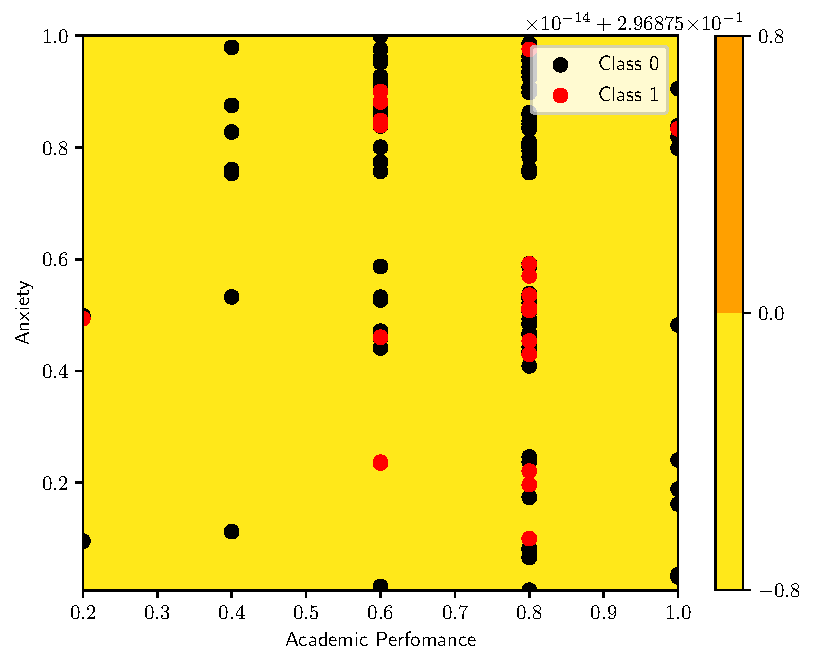
\includegraphics[width=\textwidth]{figs/tree-contour-1-4.pdf}
        \caption{}
    \end{subfigure}
    \begin{subfigure}[b]{0.32\textwidth}
        \centering
        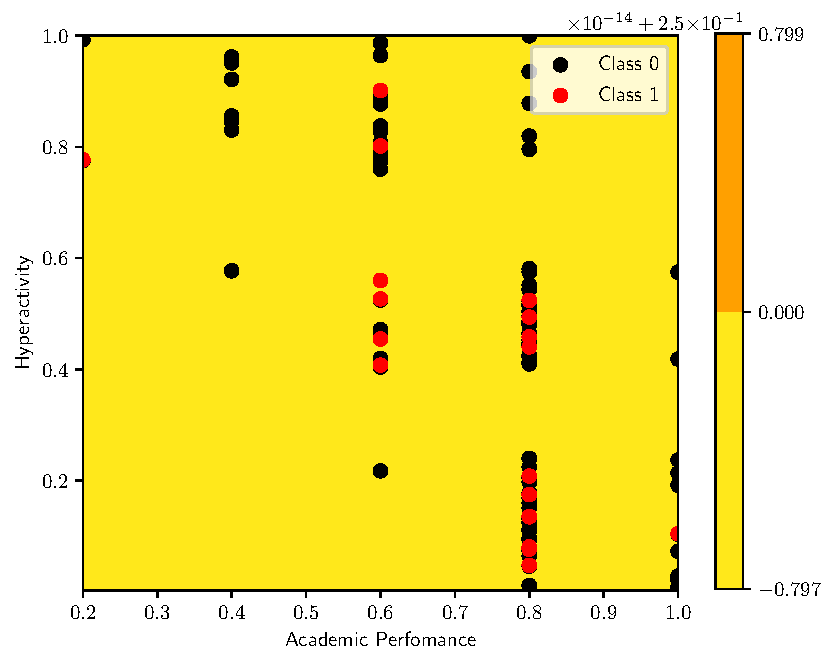
\includegraphics[width=\textwidth]{figs/tree-contour-1-5.pdf}
        \caption{}
    \end{subfigure}

    \begin{subfigure}[b]{0.32\textwidth}
        \centering
        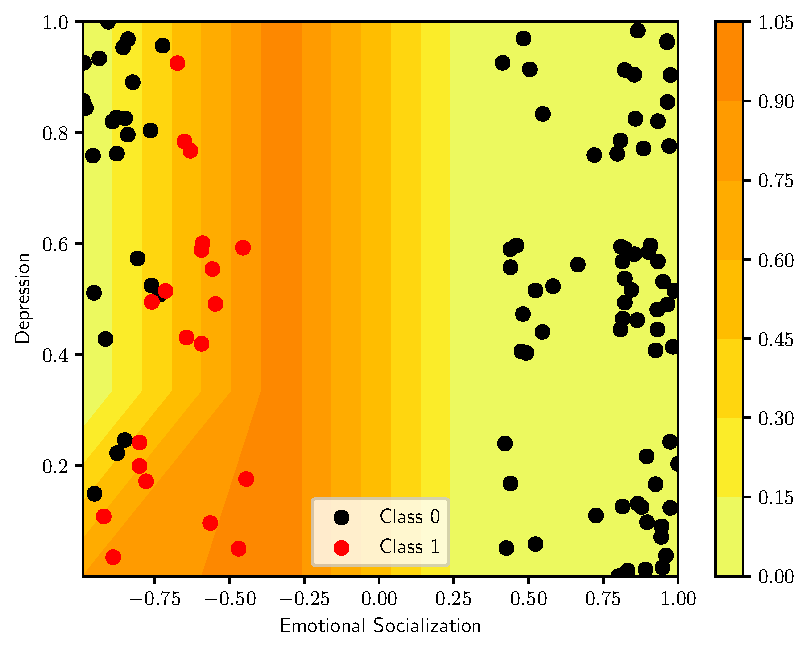
\includegraphics[width=\textwidth]{figs/tree-contour-2-3.pdf}
        \caption{}
    \end{subfigure}
    \begin{subfigure}[b]{0.32\textwidth}
        \centering
        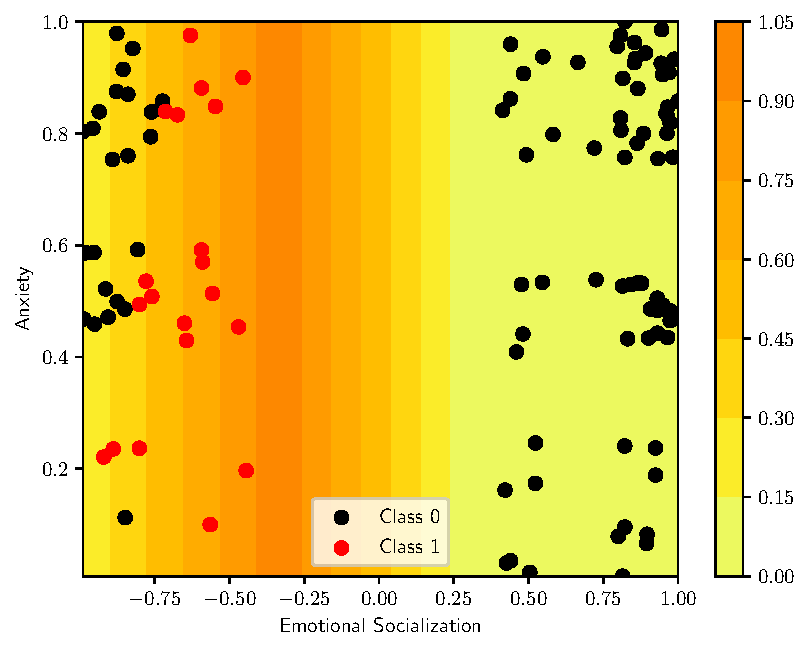
\includegraphics[width=\textwidth]{figs/tree-contour-2-4.pdf}
        \caption{}
    \end{subfigure}
    \begin{subfigure}[b]{0.32\textwidth}
        \centering
        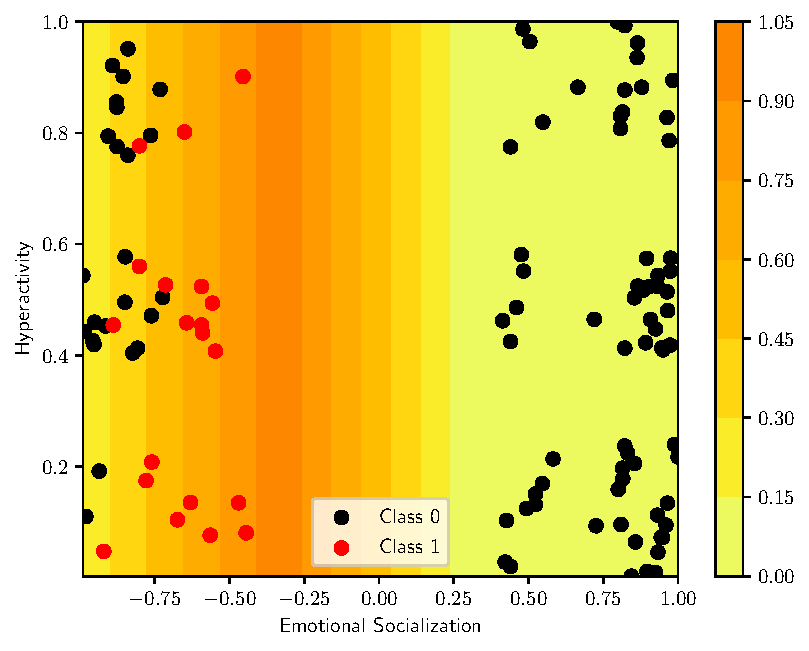
\includegraphics[width=\textwidth]{figs/tree-contour-2-5.pdf}
        \caption{}
    \end{subfigure}
    \caption{Decision Tree contour with real labels.}
    \label{fig:dts}
\end{figure*}


\subsection{Neural Networks}
\begin{figure*}
    \centering
    \begin{subfigure}[b]{0.32\textwidth}
        \centering
        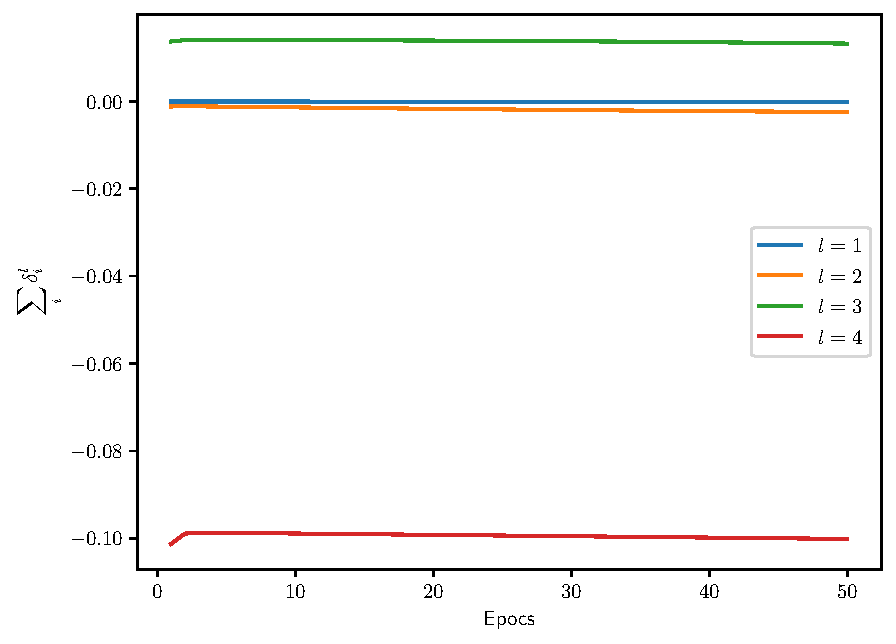
\includegraphics[width=\textwidth]{figs/1-2-3-0.9-gradients.pdf}
        \caption{Gradients for each layer.}
    \end{subfigure}
    \begin{subfigure}[b]{0.32\textwidth}
        \centering
        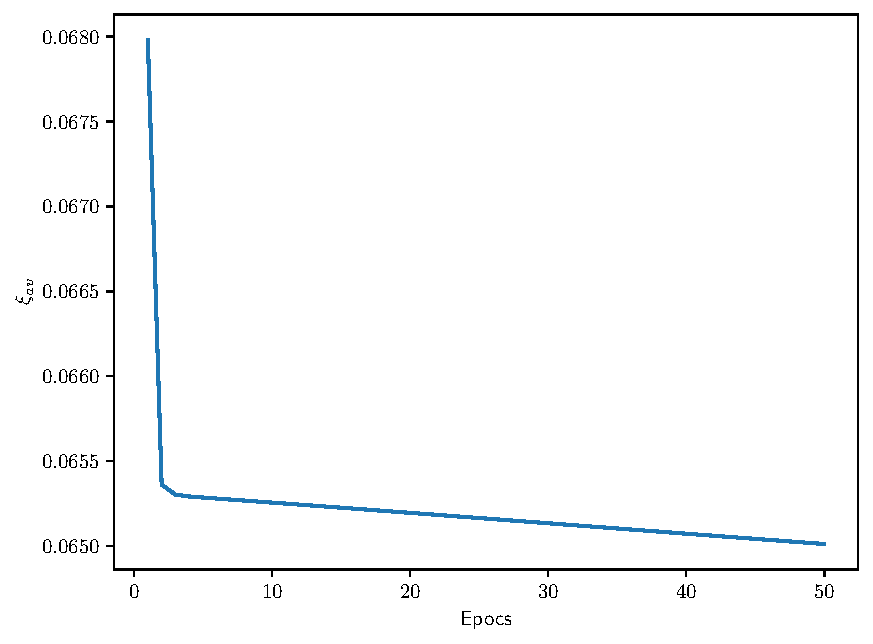
\includegraphics[width=\textwidth]{figs/1-2-3-0.9-error.pdf}
        \caption{Average error energy per epoch.}
    \end{subfigure}
    \begin{subfigure}[b]{0.32\textwidth}
        \centering
        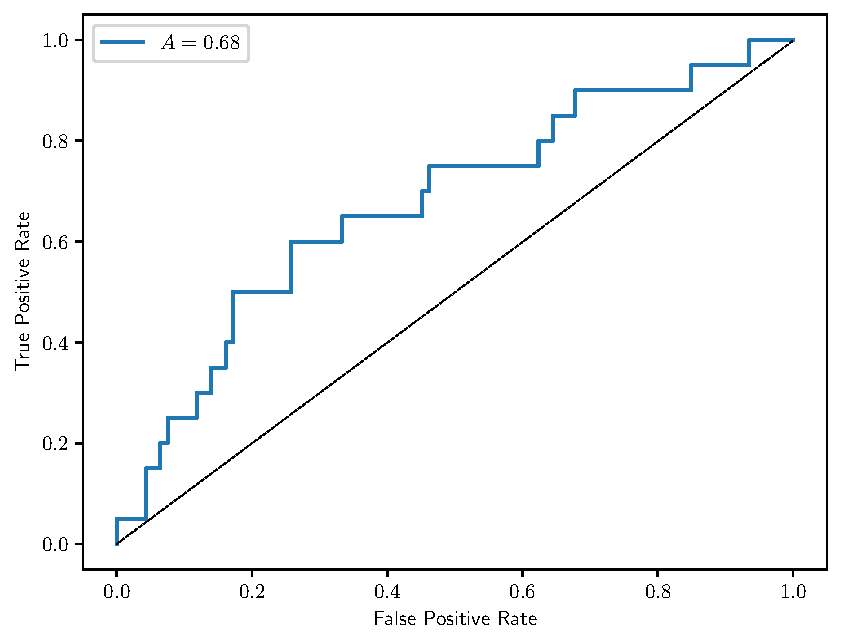
\includegraphics[width=\textwidth]{figs/1-2-3-0.9-roc.pdf}
        \caption{ROC curve.}
    \end{subfigure}
    \caption{Learning curves for $\mathcal{L}=[1,2,3]$ network $\eta=0.9$
    (worst).}
    \label{fig:NN-worst}
\end{figure*}

\begin{figure*}
    \centering
    \begin{subfigure}[b]{0.32\textwidth}
        \centering
        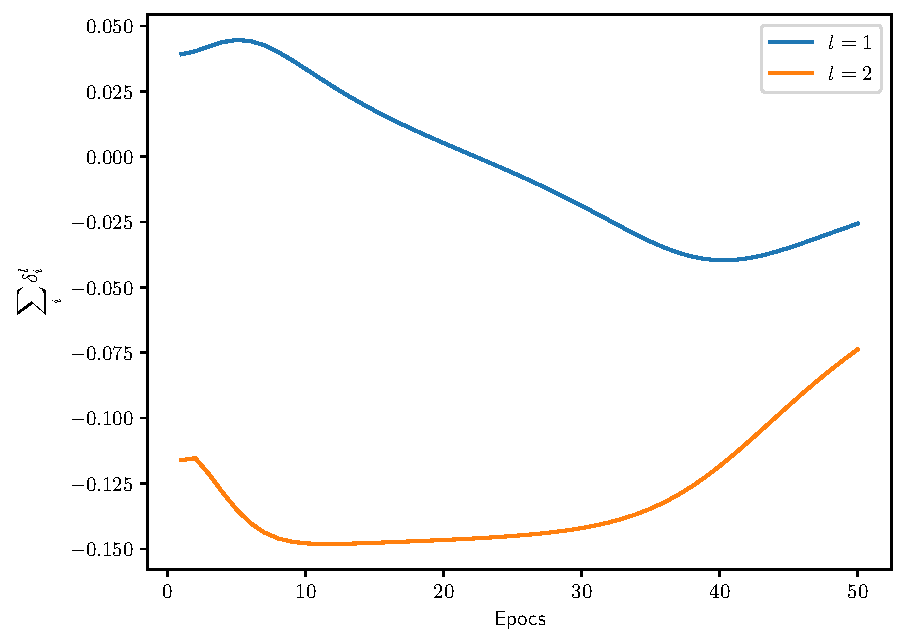
\includegraphics[width=\textwidth]{figs/2-0.9-gradients.pdf}
        \caption{Gradients for each layer.}
    \end{subfigure}
    \begin{subfigure}[b]{0.32\textwidth}
        \centering
        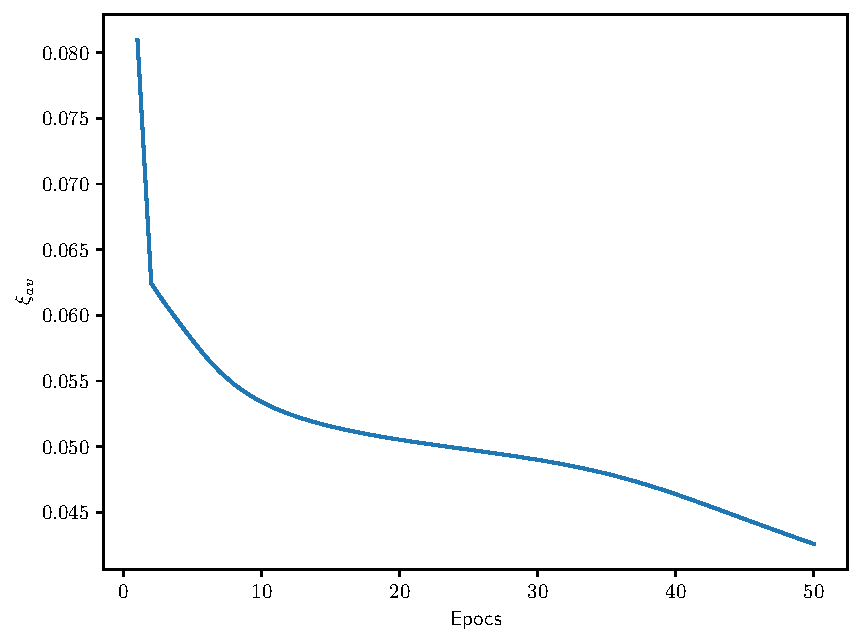
\includegraphics[width=\textwidth]{figs/2-0.9-error.pdf}
        \caption{Average error energy per epoch.}
    \end{subfigure}
    \begin{subfigure}[b]{0.32\textwidth}
        \centering
        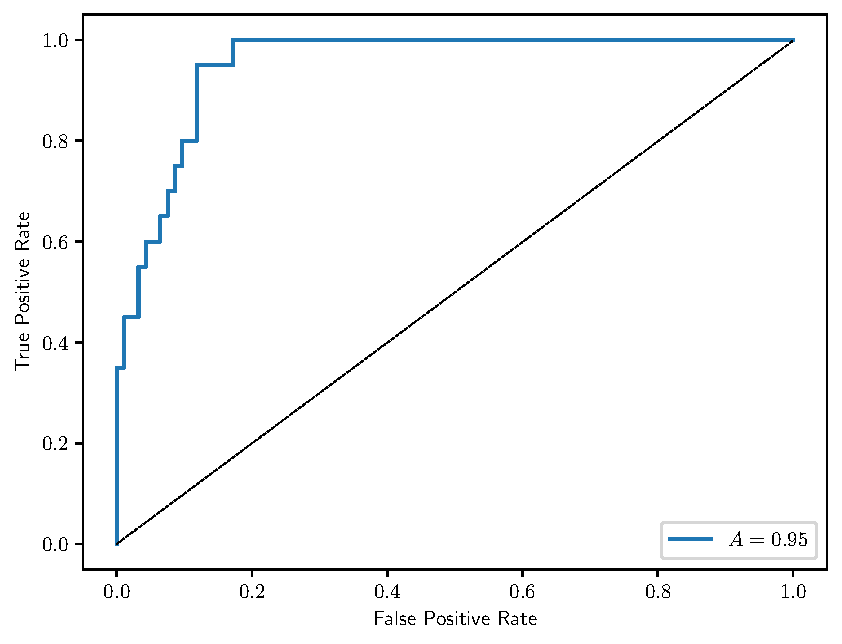
\includegraphics[width=\textwidth]{figs/2-0.9-roc.pdf}
        \caption{ROC curve.}
    \end{subfigure}
    \caption{Learning curves for $\mathcal{L}=[2]$ network with $\eta=0.9$
     (2nd best).}
    \label{fig:NN-2best}
\end{figure*}

\begin{figure*}
    \centering
    \begin{subfigure}[b]{0.32\textwidth}
        \centering
        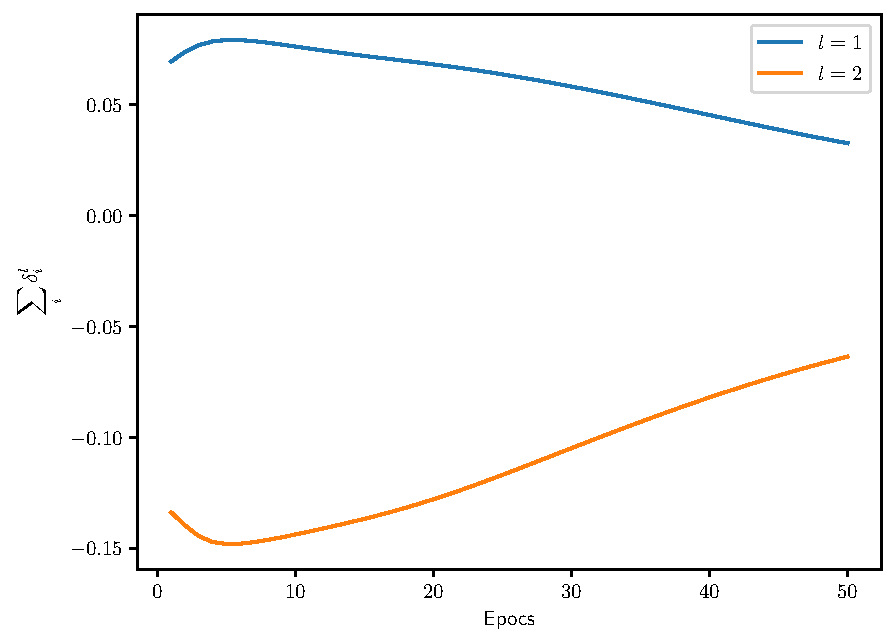
\includegraphics[width=\textwidth]{figs/3-0.9-gradients.pdf}
        \caption{Gradients for each layer.}
    \end{subfigure}
    \begin{subfigure}[b]{0.32\textwidth}
        \centering
        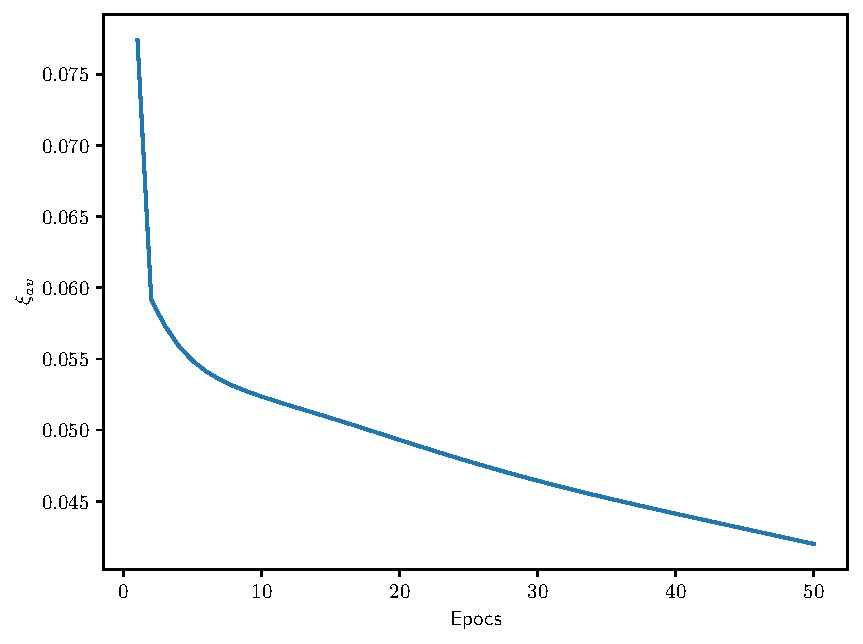
\includegraphics[width=\textwidth]{figs/3-0.9-error.pdf}
        \caption{Average error energy per epoch.}
    \end{subfigure}
    \begin{subfigure}[b]{0.32\textwidth}
        \centering
        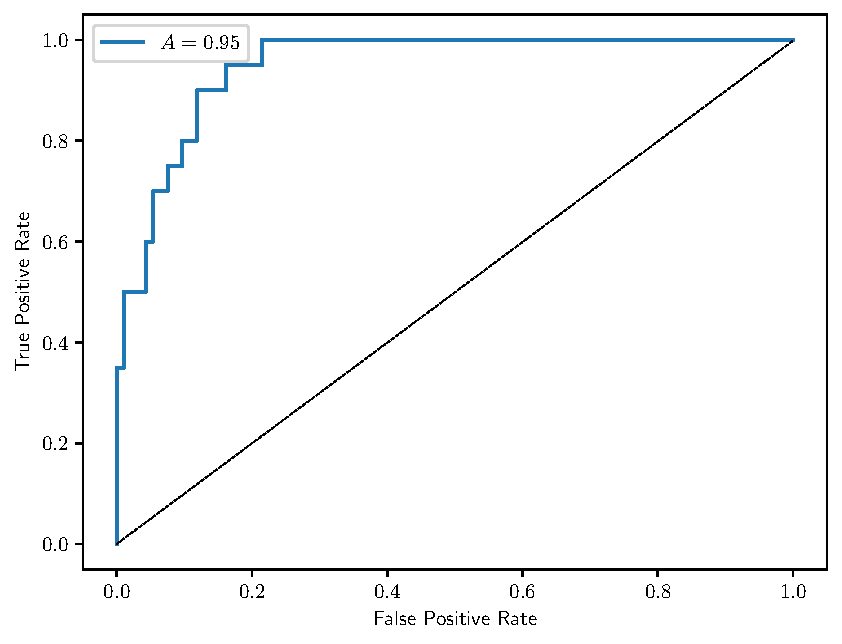
\includegraphics[width=\textwidth]{figs/3-0.9-roc.pdf}
        \caption{ROC curve.}
    \end{subfigure}
    \caption{Learning curves for $\mathcal{L}=[3]$ network with $\eta=0.9$
    (best).}
    \label{fig:NN-best}
\end{figure*}

\section{Conclusions}\label{sec:conc}

\printbibliography

\appendices

\section{Results for Embedded Data}
This section presents the same results above presented but for the data
embedded with the TSNE algorithm prior to training.
\subsection{Support Vector Machines}

\subsection{Decision Tree}
\begin{figure}
    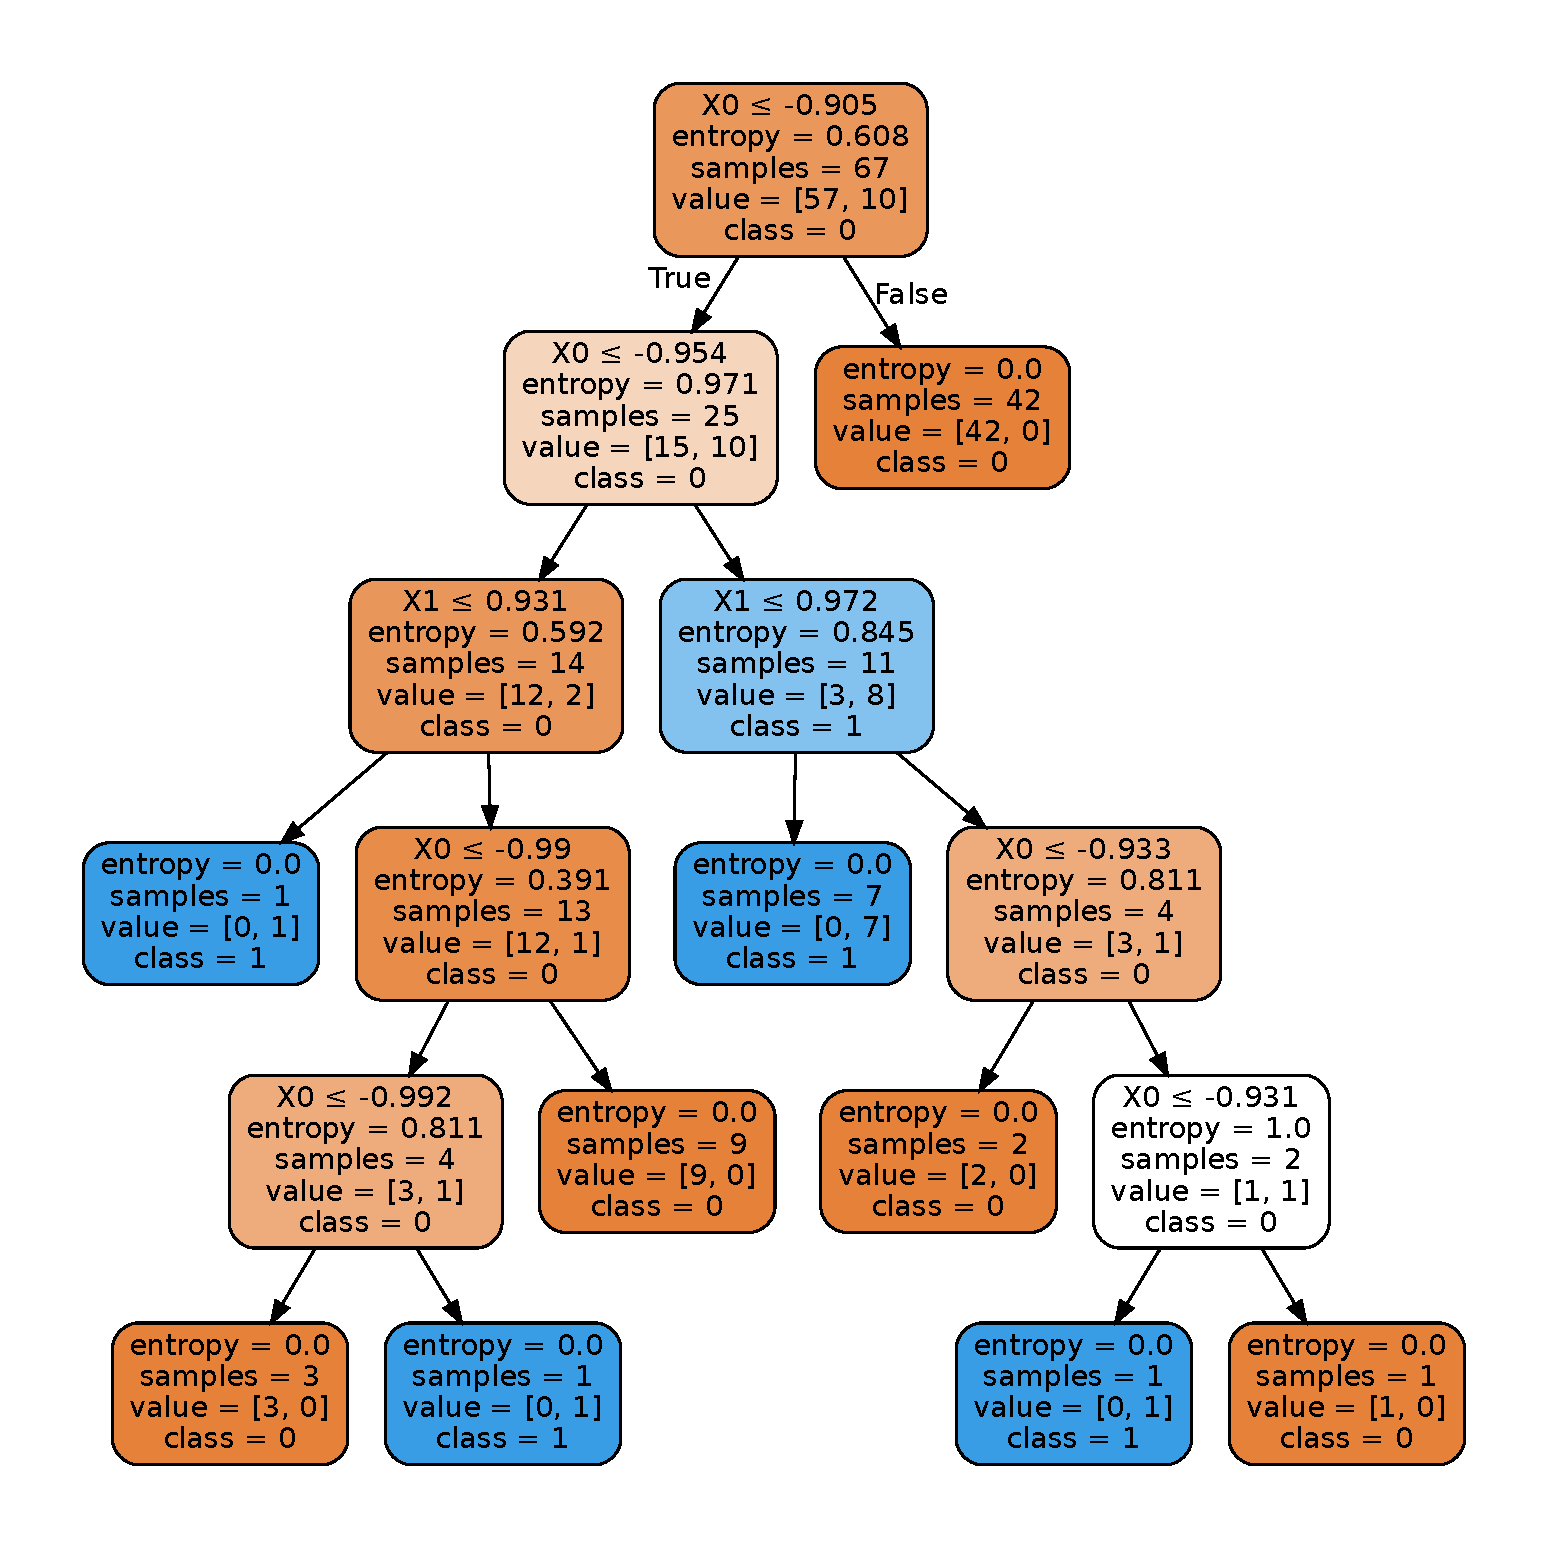
\includegraphics[width=\columnwidth]{figs/tree-emb-graph.pdf}
    \caption{Decision tree.}
    \label{fig:dte}
\end{figure}

\begin{figure}
    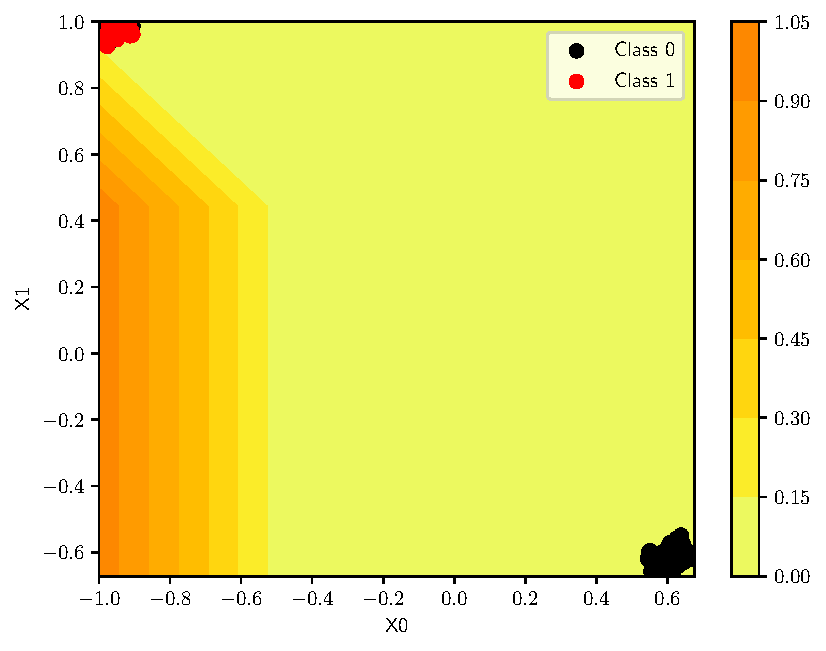
\includegraphics[width=\columnwidth]{figs/tree-contour-0-1.pdf}
    \caption{Decision Tree contour with real labels (embedded data).}
    \label{fig:dte_cont}
\end{figure}

\subsection{Neural Networks}
\begin{figure*}
    \centering
    \begin{subfigure}[b]{0.32\textwidth}
        \centering
        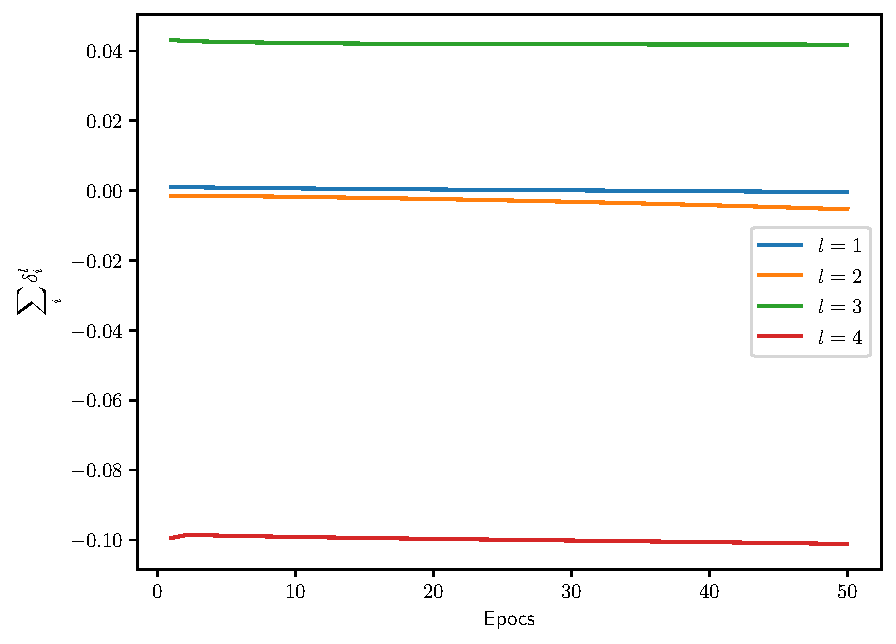
\includegraphics[width=\textwidth]{figs/2-3-3-0.9-emb-gradients.pdf}
        \caption{Gradients for each layer.}
    \end{subfigure}
    \begin{subfigure}[b]{0.32\textwidth}
        \centering
        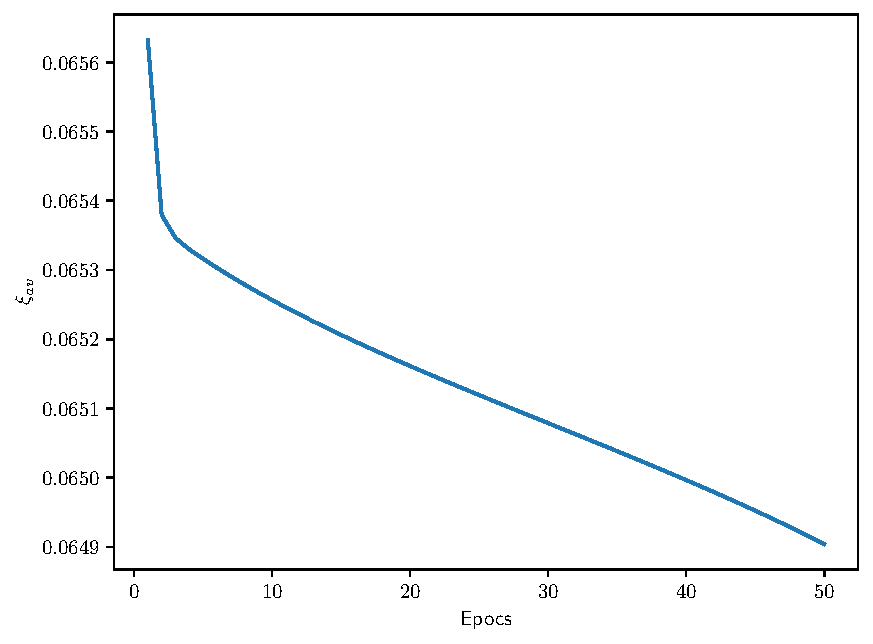
\includegraphics[width=\textwidth]{figs/2-3-3-0.9-emb-error.pdf}
        \caption{Average error energy per epoch.}
    \end{subfigure}
    \begin{subfigure}[b]{0.32\textwidth}
        \centering
        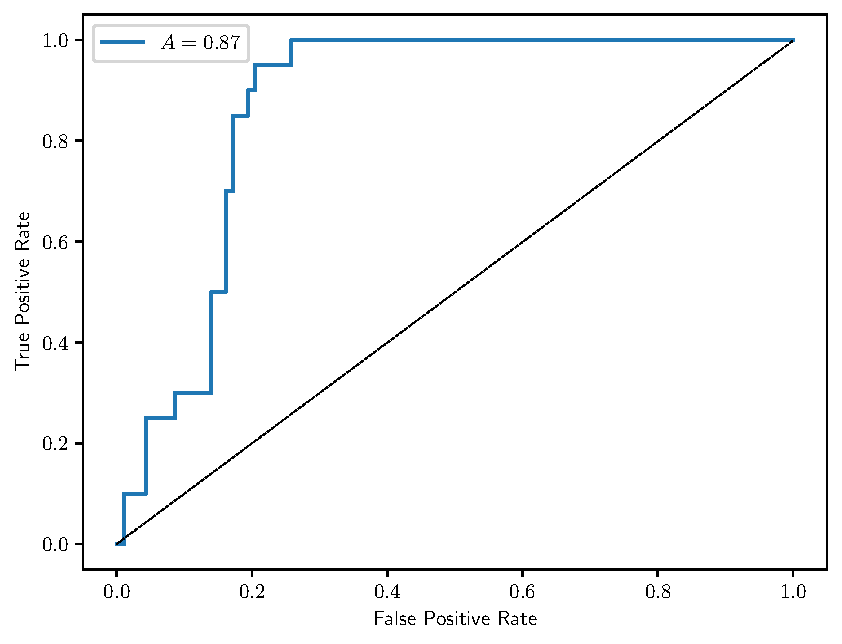
\includegraphics[width=\textwidth]{figs/2-3-3-0.9-emb-roc.pdf}
        \caption{ROC curve.}
    \end{subfigure}
    \caption{Learning curves for $\mathcal{L}=[2,3,3]$ network with $\eta=0.9$
    (worst).}
    \label{fig:NN-emb-worst}
\end{figure*}

\begin{figure*}
    \centering
    \begin{subfigure}[b]{0.32\textwidth}
        \centering
        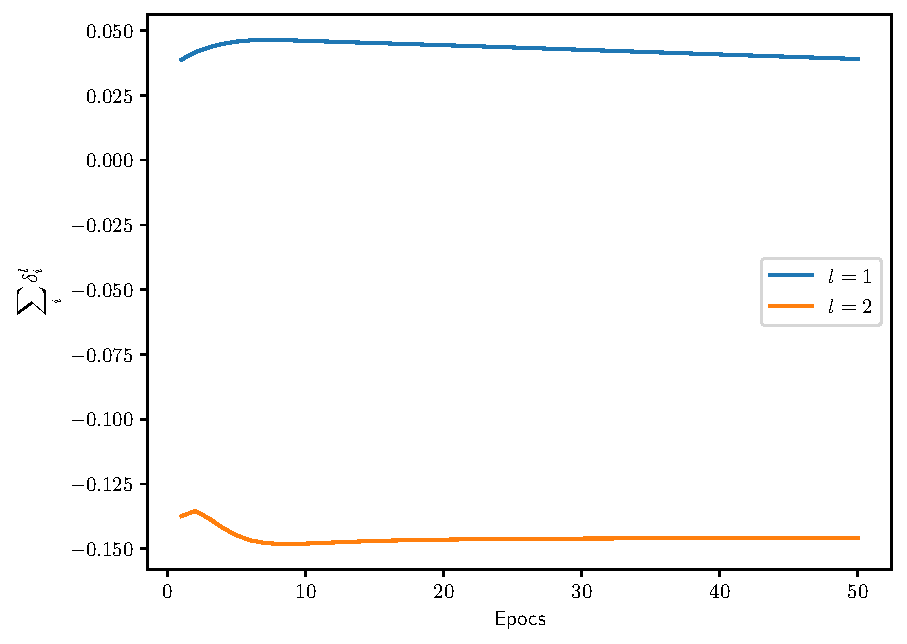
\includegraphics[width=\textwidth]{figs/3-0.5-emb-gradients.pdf}
        \caption{Gradients for each layer.}
    \end{subfigure}
    \begin{subfigure}[b]{0.32\textwidth}
        \centering
        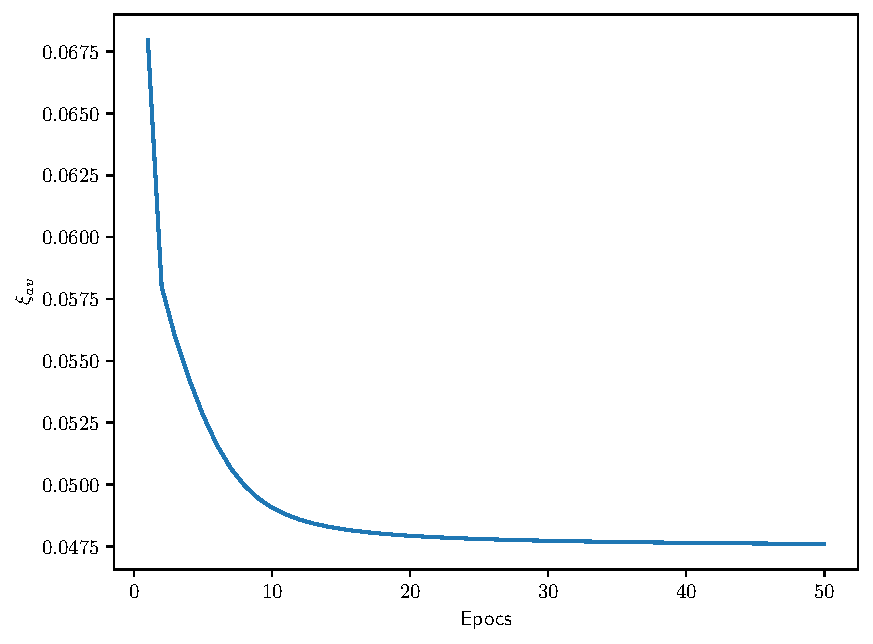
\includegraphics[width=\textwidth]{figs/3-0.5-emb-error.pdf}
        \caption{Average error energy per epoch.}
    \end{subfigure}
    \begin{subfigure}[b]{0.32\textwidth}
        \centering
        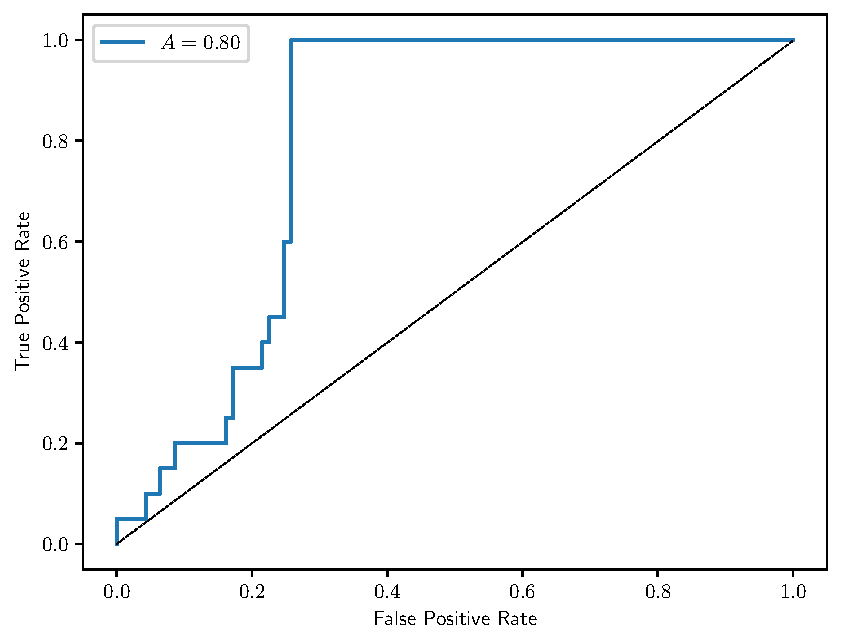
\includegraphics[width=\textwidth]{figs/3-0.5-emb-roc.pdf}
        \caption{ROC curve.}
    \end{subfigure}
    \caption{Learning curves for $\mathcal{L}=[3]$ with $\eta=0.5$ network
    (2nd best).}
    \label{fig:NN-emb-2best}
\end{figure*}

\begin{figure*}
    \centering
    \begin{subfigure}[b]{0.32\textwidth}
        \centering
        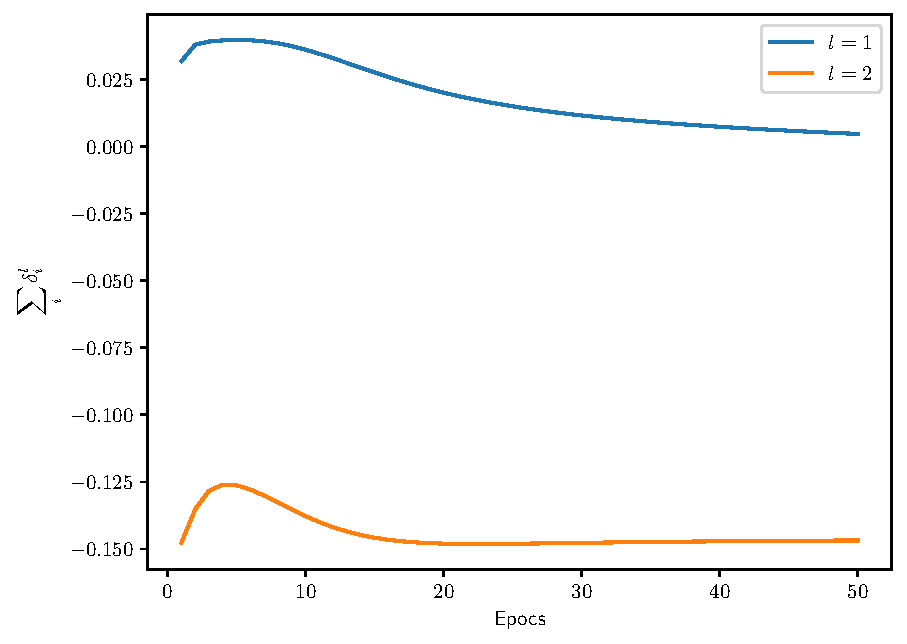
\includegraphics[width=\textwidth]{figs/2-0.2-emb-gradients.pdf}
        \caption{Gradients for each layer.}
    \end{subfigure}
    \begin{subfigure}[b]{0.32\textwidth}
        \centering
        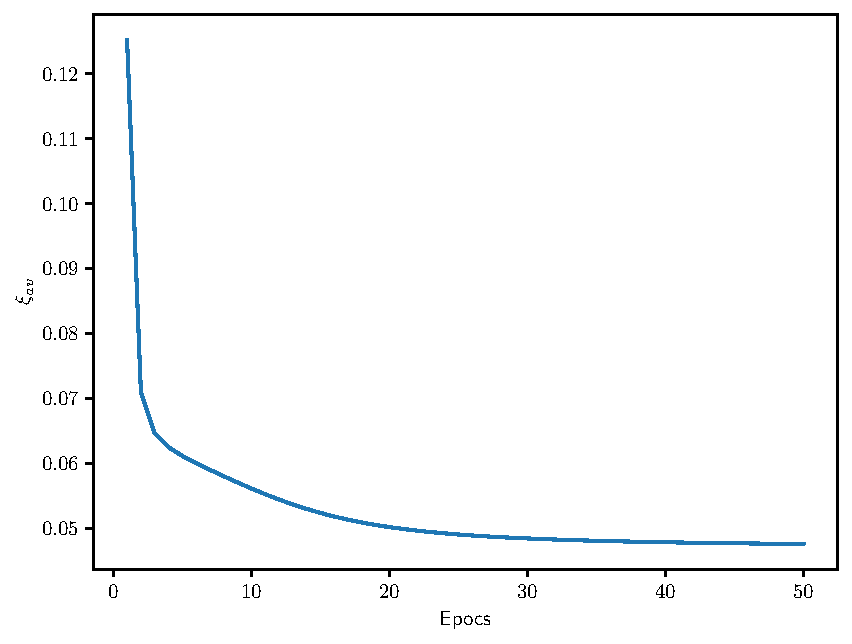
\includegraphics[width=\textwidth]{figs/2-0.2-emb-error.pdf}
        \caption{Average error energy per epoch.}
    \end{subfigure}
    \begin{subfigure}[b]{0.32\textwidth}
        \centering
        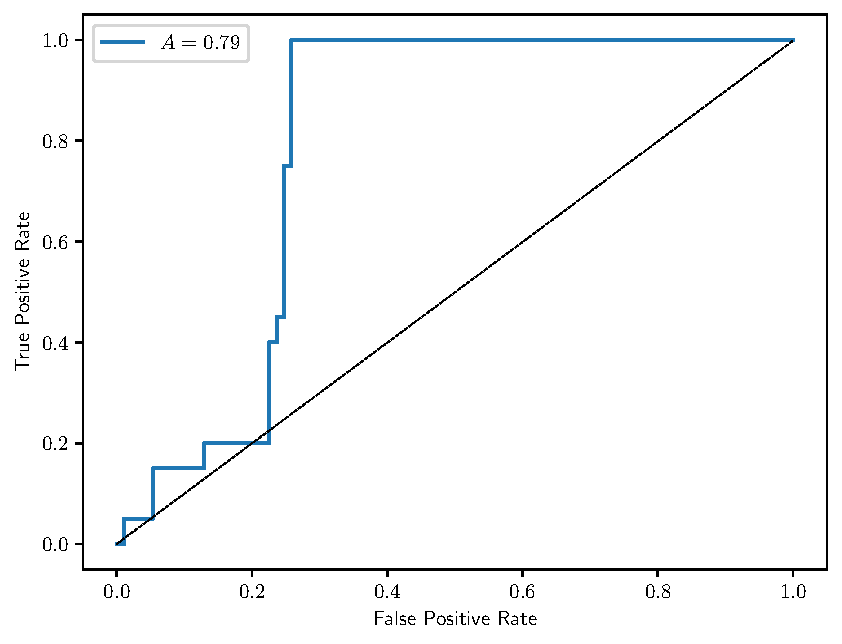
\includegraphics[width=\textwidth]{figs/2-0.2-emb-roc.pdf}
        \caption{ROC curve.}
    \end{subfigure}
    \caption{Learning curves for $\mathcal{L}=[2]$ with $\eta=0.2$ network
    (best).}
    \label{fig:NN-emb-best}
\end{figure*}

\end{document}
